\documentclass[11pt]{article}

\usepackage{exscale}
\usepackage{graphicx}
\usepackage{amsmath}
\usepackage{latexsym}
\usepackage{times,mathptm}
\usepackage{epsfig}
\usepackage{setspace}

\textwidth 6.5truein          
\textheight 9.0truein
\oddsidemargin 0.0in
\topmargin -0.6in

\parindent 0pt          
\parskip 5pt
\def\baselinestretch{1.1}

\begin{document}

\begin{LARGE}
\centerline {\bf CSci 423 Homework 3}
\end{LARGE}
\vskip 0.25cm

\centerline{Due: 1:00 pm, Wednesday, 9/26}
\centerline{Eric Shih}

\begin{enumerate}
 \item (8 points) Exercise 1.12 on page 85.
  \begin{center}
    $b(bb)^*(aa)^*$ \\
    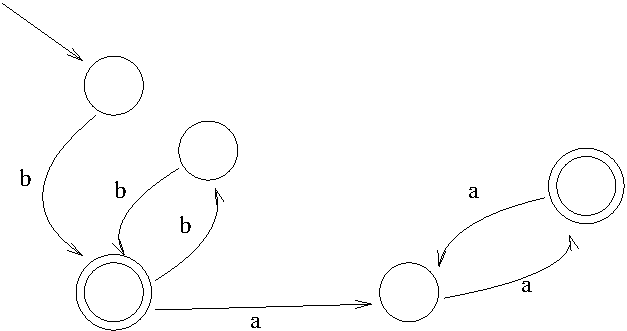
\includegraphics[scale=.4] {fig1.pdf}
  \end{center}

 \item (4 points each) Exercise 1.18 (e) (f) (j) on page 86.
  \begin{description}
   \item e. $(0 \cup 1 (0 \cup 1)) ((0 \cup 1)(0 \cup 1))^*$
   \item f. $(0^* (10^+ ))1^* $
   \item j. $00^+ \cup 100^+ \cup 0^+ 10^+ \cup 00^+1 $
  \end{description}

 \item (10 points) Exercise 1.21(b) on page 86. (Remove the states in the order of 1, 2, and 3.)
  \begin{description}
    \item a) 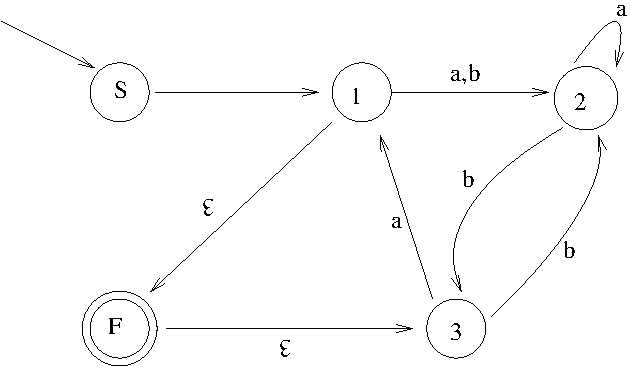
\includegraphics[scale=.4] {fig2.pdf}
    \item b) 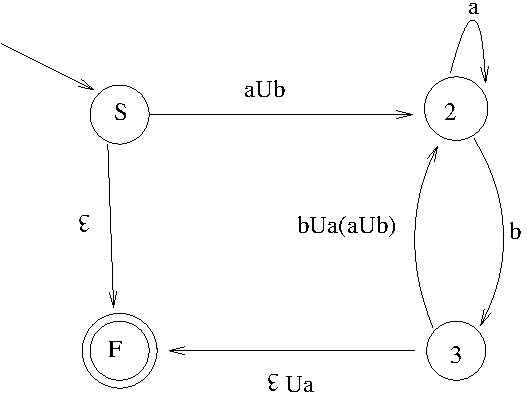
\includegraphics[scale=.4] {fig3.pdf}
    \item c) 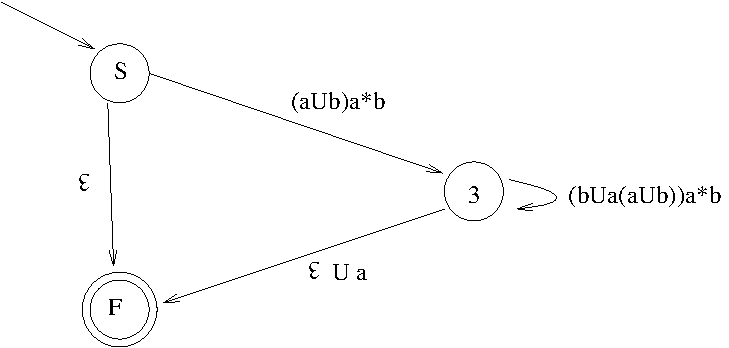
\includegraphics[scale=.4] {fig4.pdf}
    \item d) 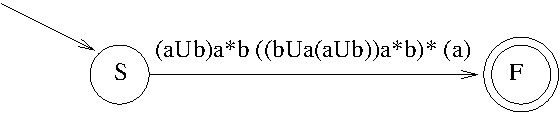
\includegraphics[scale=.4] {fig5.pdf}
  \end{description}

 \item (5 points) Problem 1.37 on page 89. *reference attained from Koether of Hampden-Sydney College*\\
  A DFA can be designed for $C_n$ by tracking the remainder of $input/n$. If input mod n is 0, we accept the state, 
  otherwise we reject it.
  \begin{description}
   \item DFA M = $(Q, {0,1}, \delta, q_0 , F)$ where: \\
    $Q = q_0 , q_1 , q_2, ... , q_{n-1}$ \\
    $\delta(q_i , 0) = q_{(2i mod n)}$ \\
    $\delta(q_i , 1) = q_{(2i+1 mod n)}$ \\
    $F = q_0$
  \end{description}


 \item (5 points) Problem 1.48 on page 90. 
  \begin{center}
    Because a DFA can be made, D is a regular language.
    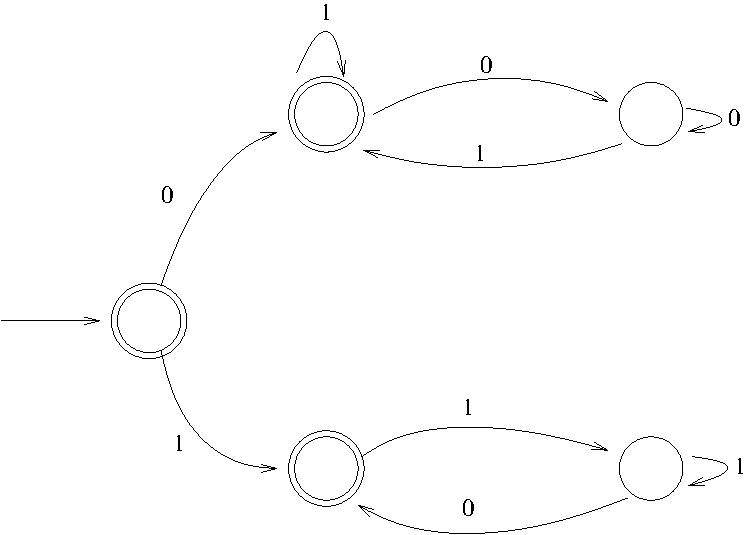
\includegraphics[scale=.9] {fig6.pdf}
  \end{center}
\end{enumerate}

\end{document}

